% !TEX root = ../main.tex

\section{Background and Analysis}
\label{sec:background}

In this section, we present the notation, setup, and assumptions on which we base the work. Additionally, we conduct an analysis of contrastive \ac{VL} representation learning with multiple captions per image.

\subsection{Preliminaries}
\label{subsec:notation-assumptions}

\header{Notation} We closely follow the notation from \citep{bleeker2023reducing}. 
See Table~\ref{tab:notation} for an overview.
Let $\mathcal{D}$ be a dataset of $N$ image-caption tuples: $\mathcal{D} = \left\{\left(\img{i}, \{\capt{i}{j}\}_{j=1}^{k} \right)\right\}_{i=1}^{N}$. 
Each tuple $i \in N$ contains one image $\img{i}$ and $k$ captions $\capt{i}{j}$, where $1 \leq j \leq k$. 
All captions in tuple $i \in N$ are considered as matching captions w.r.t.\ image $\img{}$ in the tuple $i$.
The latent representation of an image-caption pair from a tuple $i$ is denoted as $\zimg{i}{}$ and $\zcapt{i}{j}$ respectively.
During training, we sample image-caption pairs from the dataset $\mathcal{D}$ and optimize for the evaluation task $T$. 
We include all captions in the dataset once per training epoch, hence, each image is sampled $k$ times.

Given an image $\img{}$, a set of $k$ associated captions $K = \{\capt{}{j}\}_{j=1}^{k}$, and one caption randomly sampled from the set $\capt{}{} \in K$,
we define the following representations:
\begin{enumerate*}[label=(\roman*)]
	\item $\zcaptsuff{}{}$ as \emph{sufficient} representation of the caption $\capt{}{}$ that describes the image $\img{}$;
	\item $\zimgsuff{}$ as representation of the image $\img{}$ \emph{sufficient for the caption} $\capt{}{}$;
	\item $\zminsuff{}$ as representation of the image $\img{}$ that is \emph{minimally sufficient for the caption} $\capt{}{}$; and
	\item $\zoptimal{}{K}$ as representation of the image $\img{}$ that is \emph{optimal for the set of captions} $K$ given the task $T$.
\end{enumerate*}

In addition, we write
$\sct{}$ for a synthetic shortcut,
$S$ for the original shared information, i.e., information that does not contain synthetic shortcuts,
$S^{+}$ for the shared information that includes a synthetic shortcut,
and $R^{+}$ for task-relevant information that contains a synthetic shortcut.

In the context of task relevance, we define $R$ and $\neg R$ as task-relevant and task-irrelevant information, respectively, and $C$ as task-relevant information specific for caption $\capt{}{}$.

\header{Setup} 
We work with a dual-encoder setup, with an image encoder and a caption encoder that do not share parameters. 
The \emph{image encoder} $f_{\theta}(\cdot)$ takes an image $\img{}$ as input and returns its latent representation: $\zimg{}{} :=  f_{\theta}(\img{})$.
Similarly, the \emph{caption encoder} $g_{\phi}(\cdot)$ takes a caption $\capt{}{}$ as input, and encodes the caption into a latent representation: $\zcapt{}{} :=  g_{\phi}(\zcapt{}{})$. 
Both $\zcapt{}{}$ and $\zimg{}{}$ are unit vectors projected into $d$-dimensional multi-modal space: $\zcapt{}{} \in \sR^d$, $\zimg{}{} \in \sR^d$.
For an overview of notation, we refer to Appendix~\ref{appendix:notation}, Table~\ref{tab:notation}.

\header{Assumptions}
Given an image-caption tuple, 
we assume that each caption in the tuple is distinct from the other captions in the tuple.
We also assume that each caption in the tuple contains two types of task-relevant information:
\begin{enumerate*}[label=(\roman*)]
	\item shared information, i.e., information shared with other captions in the same tuple,
	and 
	\item caption-specific information, i.e., information that is not shared with the other captions.
\end{enumerate*}
For simplicity, we base our subsequent analysis on tuples where one image $\img{}{}$ is associated with two captions $\capt{}{A}$ and $\capt{}{B}$: $\left(\img{}, \{\capt{}{A}, \capt{}{B}\} \right)$. 
However, the analysis described in this section can be extended to a case with more than two captions. We treat images and captions as views and define  $\img{}{}$, $\capt{}{A}$, and $\capt{}{B}$ to be random variables of an image and two matching captions, with the joint distribution $p(\img{}{}, \capt{}{A}, \capt{}{B})$.
For more details on assumptions and problem definition, we refer to Appendix~\ref{appendix:problem}.

\subsection{Analysis of Contrastive Vision-Language Representation Learning for Multiple Captions per Image}

\header{InfoMax} We start our analysis of contrastive \ac{VL} representation learning by introducing the InfoMax optimization objective, a typical loss for \ac{VL} representation learning.
The goal of an InfoMax optimization objective, e.g., InfoNCE~\citep{oord2018representation}, is to maximize the \ac{MI} between the latent representations of two views of the same data~\citep{tschannen2020on}. 
Therefore, the optimization objective is equivalent to: $ \max_{f_{\theta}, g_{\phi} } I (\zimg{}{} ; \zcapt{}{} ) $ where $\zimg{} := f_{\theta}(\img{}{})$ and $\zcapt{}{} := g_{\phi}(\capt{}{})$.
%\ay{This definition of task-relevant seems fine for our purposes (and I guess follows prior work), but I think it's really about the dataset rather than the task? It's about the information that exists in a set of existing queries, not about the (many) queries that could reasonably be asked given the task.}


\header{Minimally Sufficient Image Representation} During training, batches of image-caption pairs are sampled. 
The optimization involves maximizing the \ac{MI} between the image representation $\zimg{}{}$ and the matching caption representation $\zcapt{}{}$.
\cite{wang2022rethinking} argue that, since all supervision information for one view (i.e., the image) comes from the other view (i.e., the caption), the representations learned contrastively are approximately minimally sufficient.
Following \citep{tian2020what, wang2022rethinking}, we extend the definition of sufficient representation to \ac{VL} context and define sufficient caption representations, sufficient image representations, and minimally sufficient image representation.

\begin{definition}[Sufficient caption representation]
	\label{def:suff_capt_repr}	
	Given an image $\img{}{}$, and a set of matching captions $\mathcal{C} = \{ \capt{}{A}, \capt{}{B} \}$,
	the representation $\zcaptsuff{}{}$ of caption $\capt{}{} \in \mathcal{C}$ is sufficient for image $\img{}{}$ if, and only if, $I(\zcaptsuff{}{}; \img{}{} ) = I(\capt{}{}; \img{}{})$.
\end{definition}
The sufficient caption representation $\zcaptsuff{}{}$ contains all the information about image $\img{}{}$ in caption $\capt{}{}$.
 
\begin{definition}[Sufficient image representation]
	\label{def:suff_img_repr}		
	Given an image $\img{}{}$, and a set of matching captions $\mathcal{C} = \{ \capt{}{A}, \capt{}{B} \}$,
	the representation $\zimgsuff{}$ of image $\img{}{}$ is sufficient for caption $\capt{}{} \in \mathcal{C}$ if, and only if,  $I(\zimgsuff{}; \capt{}{} ) = I(\img{}{} ; \capt{}{})$.
\end{definition}

Similarly, the sufficient image representation $\zimgsuff{}$ contains all the shared information between an image $\img{}{}$ and a caption $\capt{}{}$. 
% We define it as \emph{pairwise} sufficient because it is defined between a single image-caption pair. 
Note that a sufficient image representation can be sufficient w.r.t.\ multiple captions.

\begin{definition}[Minimally sufficient image representation]
	\label{def:zimgminsuff}		
	Given an image $\img{}{}$, and a set of matching captions $\mathcal{C} = \{ \capt{}{A}, \capt{}{B} \}$,
	the sufficient image representation $\zminsuff{}$ of image $\img{}{}$  is minimally sufficient for caption $\capt{}{} \in \mathcal{C}$ if, and only if, $I(\zminsuff{}; \img{}{}) \leq I(\zimgsuff{}; \img{}{})$, for all $\zimgsuff{}$ that are sufficient.
\end{definition}
Intuitively, $\zminsuff{}$ comprises the smallest amount of information about $\img{}{}$ (while still being sufficient) and, therefore, only contains the information that is shared with caption $\capt{}{}$, i.e., the non-shared information is suppressed.
% Since we assume that everything in the caption is relevant w.r.t.\ the image it describes (see Assumption~\ref{asm:1}), a sufficient caption representation $\zcaptsuff{}{}$ is minimally sufficient.  

\begin{figure*}[t!]
	\centering
	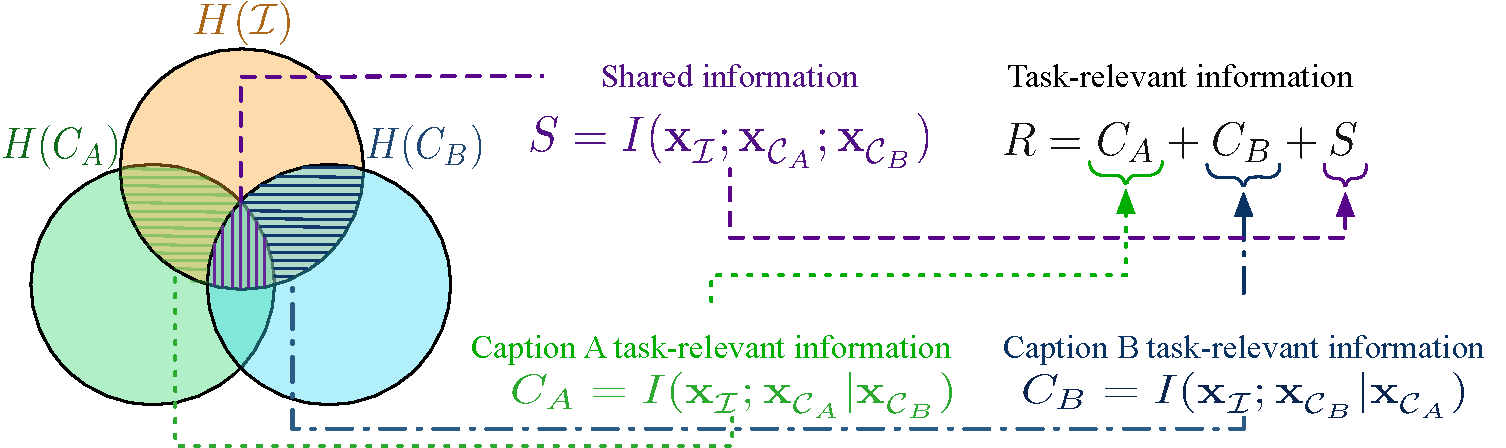
\includegraphics[width=0.85\textwidth]{figures/information-venn-diagram}
	\caption{
		We define $H(\img{}{})$ as image information, $H(\capt{}{A})$ and $H(\capt{}{B})$ as caption information;
		both captions only describe the information depicted in the image and contain shared and caption-specific information.
		We further define
		$C_A = I( \img{}{} ; \capt{}{A} \mid \capt{}{B})$
		and
		$C_B = I( \img{}{} ; \capt{}{B} \mid \capt{}{A})$ as caption-specific information; 
		$S = I(\img{}{} ; \capt{}{A} ; \capt{}{B})$ as shared information;
		$\neg R = H( \img{}{} \mid \capt{}{A} , \capt{}{B} ) $ as task-irrelevant information;
		$R = C_A + C_B + S$ as task-relevant information.
	}
	\label{fig:venn}
\end{figure*} 

\header{Task-Optimal Image Representation} The definition of task-optimal image representation is based on the notion of task-relevant information. 
In the context of \ac{VL} representation learning with multiple captions per image, we define task-relevant information as all information described by the matching captions. That includes both caption-specific and shared information.
Consequently, task-optimal image representation is image representation that is sufficient w.r.t. all matching captions.

Formally, following assumptions from Appendix~\ref{app:assumptions}, we define task-relevant information $R$ as all the information described by the matching captions. The task-relevant information can be expressed as follows:
%
\begin{equation}
\begin{split}
	\underbrace{R}_{\substack{\text{Task-relevant}\\ \text{information}}} & =
	\underbrace{H(\img{}{} )}_{\substack{\text{Image}\\ \text{information}}}
	- \underbrace{H(\img{}{} \mid \capt{}{A} , \capt{}{B})}_{\substack{\text{Task-irrelevant}\\ \text{information}}}
	\\
	& = 
	\underbrace{I( \img{}{} ; \capt{}{A} \mid \capt{}{B})}_{\substack{\text{$C_{A}$-specific}\\ \text{task-relevant information}}}
	+
	\underbrace{I( \img{}{} ; \capt{}{B} \mid \capt{}{A})}_{\substack{\text{$C_{B}$-specific}\\ \text{task-relevant information}}}
	+
	\underbrace{I(\img{}{} ; \capt{}{A};\capt{}{B})}_{\substack{\text{Shared}\\ \text{information}}}.
\end{split}	
	\label{eq:task_relevant}
\end{equation}
%
Similarly, task-irrelevant information $\neg R$ is the image information not described by the captions. Figure~\ref{fig:venn} illustrates both definitions.

The multi-view assumption states that task-relevant information for downstream tasks comes from the information shared between views~\citep{shwartz2023compress}.  
However, in the case of \ac{VL} representation learning with multiple captions per image, task-relevant information $R$ includes both shared information $S$, and caption-specific information $C_A$ and $C_B$ (Eq.~\ref{eq:task_relevant}).

\begin{definition}[Task-optimal image representation]
	\label{def:opt_z}	
	Given an image $\img{}{}$, and a set of matching captions $\mathcal{C} = \{ \capt{}{A}, \capt{}{B} \}$, 
	the representation $\zoptimal{}{\mathcal{C}}$ is task-optimal image representation for all matching captions if, and only if, $I(\zoptimal{}{\mathcal{C}}; \capt{}{}) = I(\img{}{}; \capt{}{})$, for all $\capt{}{} \in \mathcal{C}$.
\end{definition}
In other words, task-optimal image representations contain all the information that the image shares with the matching captions. 
Hence, a task-optimal image representation is sufficient w.r.t.\ all matching captions. 
The information contained in the task-optimal image representation includes both shared and caption-specific information.
Therefore, a task-optimal image representation can never be a minimally sufficient image representation w.r.t.\ to a specific caption.

\begin{thm}{1}[Suboptimality of contrastive learning with multiple captions per image]
	\label{thm:suboptimality-main}	
	Given an image $\img{}{}$, a set of matching captions $\mathcal{C} = \{ \capt{}{A}, \capt{}{B} \}$, and a contrastive learning loss function $\infonce{}$ that optimizes for task $T$, 
	image representations learned during contrastive learning will be minimally sufficient and will never be task-optimal image representations.
\end{thm}

The proof is provided in Appendix~\ref{app:analysis-of-contrastive}.
Rephrasing Theorem~\ref{thm:suboptimality-main}, given an image and two captions that form two image-caption pairs, $(\img{}{}, \capt{}{A})$ and $(\img{}{}, \capt{}{B})$, and assuming that contrastive loss optimizes the image encoder to be minimally sufficient w.r.t.\ to caption $\capt{}{A}$ during a training step, all task-relevant information $C_{B}$ specific to caption $\capt{}{B}$ will be suppressed in $\zimg{}{}$. Hence, the resulting image representation will not be optimal for the task $T$.

Theorem~\ref{thm:suboptimality-main} indicates a discrepancy between minimally sufficient representations learned during contrastive training with the InfoNCE loss and the task-optimal image representations in the context of learning \ac{VL} representations with multiple captions per image.
Although the InfoMax loss does not have an explicit constraint to compress information, prior work indicates that feature suppression is happening \citep{shwartz2023compress, robinson2021can}. 
Hence, we question if contrastive loss can be used to learn task-optimal image representations in the context of multiple captions per image.

Furthermore, Theorem~\ref{thm:suboptimality-main} implies that in the context of contrastive \ac{VL} representation learning with multiple captions per image, the minimally sufficient representation, which discards non-shared information, is not the same as the task-optimal representation that comprises both caption-specific and shared information.  
This suggests that the features learned during contrastive learning might be shortcuts, i.e., easy-to-detect discriminatory features that minimize the contrastive optimization objective but are not necessarily sufficient for solving the evaluation task.
To examine this problem, we introduce a synthetic shortcuts framework that allows us to investigate the problem of suboptimality of contrastive learning with multiple captions per image in a controlled way.